% SABER AAAI-27 Korean submission skeleton.
% This file is intentionally separated from saber_aaai27_draft_kr.tex.
% Goal: keep the main submission self-contained and close to AAAI page limits.
% English page-limited submission skeleton.

\documentclass[letterpaper]{article}
\usepackage[submission]{aaai2027}
\usepackage[hyphens]{url}
\usepackage{graphicx}
\graphicspath{{./}{../}}
\urlstyle{rm}
\def\UrlFont{\rm}
\usepackage{natbib}
\usepackage{caption}
\frenchspacing

\usepackage{amsmath}
\usepackage{amssymb}
\usepackage{booktabs}
\usepackage{array}

\ifdefined\pdfinfo
\pdfinfo{
/TemplateVersion (2027.1)
}
\fi

\setcounter{secnumdepth}{2}
\setcounter{dbltopnumber}{3}
\renewcommand{\dbltopfraction}{0.95}
\renewcommand{\textfraction}{0.05}

\newcommand{\ours}[1]{\textbf{#1 (Ours)}}
\newcommand{\oursnum}[1]{\(\boldsymbol{#1}\)}
\newcommand{\ourscell}[1]{\textbf{#1}}

\title{SABER: Support-Conditioned Adaptive Bellman Error Reweighting for Sparse HER Actor-Critic}
\author{Anonymous Submission}
\affiliations{}

\begin{document}
\maketitle

\begin{center}
\small\textbf{Content Areas:}\\
ML: Reinforcement, Imitation \& Inverse RL (primary);\\
ROB: Robot Learning, Control \& Foundation Models (secondary)
\end{center}
% Keep these labels synchronized with the OpenReview selections and add the paper ID once assigned.

\begin{abstract}
Hindsight Experience Replay (HER) relabels failed trajectories with achieved goals; most extensions modify goal, transition, or target selection. We study whether critic residuals should remain equally weighted once relabeling and sampling are fixed. SABER (Support-Conditioned Adaptive Bellman Error Reweighting), a critic-only objective, upweights a Bellman residual when replay actions from a sufficiently populated, discretized state-goal-horizon context occupy the current-policy action bin. It normalizes weights to mean one per minibatch while leaving HER relabeling, uniform replay, actor losses, Bellman targets, architectures, and the update-to-data (UTD) ratio unchanged. Under matched UTD-1 FetchPickAndPlace training, mean normalized success AUD rises across DDPG, TD3, and SAC; 95\% confidence intervals for paired differences lie entirely above zero for TD3 and SAC but include zero for DDPG. Extending the TD3 protocol to 10 seeds yields a paired AUC gain of \(+0.0467\) (95\% CI \([0.0085, 0.0783]\)), with SABER outperforming HER in 8 of 10 seeds. On DrawerOpen with DDPG, mean AUC rises from \(0.207\) to \(0.754\), and mean final success from \(0.390\) to \(1.000\). In a matched FPP TD3 ablation changing only the support query, the current-policy query exceeds replay-action and sample-shuffled policy queries by \(+0.075\) and \(+0.096\) AUC, respectively. A stricter control randomly upweights an equal number of samples from  the same context-eligible set; the SABER-minus-control AUC estimate is \(+0.052\), but its 95\% CI includes zero, although SABER outperforms it in 4 of 5 seeds. Together, the results identify post-HER critic-loss allocation as a distinct, conditionally useful axis, while exact support membership's independent causal contribution remains unresolved.
\end{abstract}

\section{Introduction}

A central challenge in sparse-reward goal-conditioned reinforcement learning is obtaining useful learning signals when successful trajectories are rare. Hindsight Experience Replay (HER) addresses this challenge by relabeling transitions from failed trajectories with achieved goals and recomputing their rewards, thereby turning otherwise unsuccessful experience into trainable goal-conditioned transitions~\citep{andrychowicz2017her}. HER therefore determines which relabeled goals and rewards are used for learning. Once replay sampling and relabeling are fixed, however, standard HER actor--critics typically minimize an equally weighted average of per-sample squared Bellman residuals. HER thus leaves a separate design question unresolved: how should critic supervision be allocated within a relabeled minibatch? This question matters because the critic regresses Bellman targets at replay actions, whereas the actor queries the critic at current-policy actions. The availability of same-context replay actions matching these policy queries can vary across samples, yet standard HER assigns the same explicit critic-loss coefficient regardless of replay-support status; we therefore study replay support only as an observable, policy-query-aligned signal, not as a guarantee of target accuracy or lower variance.

We introduce SABER (Support-Conditioned Adaptive Bellman Error Reweighting) to isolate this post-HER design axis. For each sampled and relabeled transition, SABER gathers replay actions sharing the same discretized state--goal--horizon context. It marks the sample as support-positive when this local set is sufficiently populated and contains a replay action in the same action bin as the current-policy action. SABER assigns raw weight \(1+\lambda_S\) to a support-positive sample and \(1\) otherwise, then normalizes the weights to have unit minibatch mean. The current-policy action is used only for this support query; Bellman regression remains evaluated at the original replay action.

SABER therefore changes only the relative coefficients of the critic's per-sample Bellman losses. It preserves HER relabeling, uniform replay sampling, recomputed rewards, Bellman targets, the actor objective, network architectures, and updates per step. This controlled intervention isolates the empirical effect of critic-loss allocation from changes to goal selection, sample inclusion, target construction, policy optimization, architecture, or update budget. We evaluate SABER under the standard one-update-per-step regime, using high-replay-ratio HER and REDQ-HER as scaling references rather than matched mechanism controls.

Our contributions are:
\begin{itemize}
    \item \textbf{Problem:} We identify post-HER critic supervision allocation as a distinct design axis from goal relabeling, replay prioritization, and Bellman-target construction.
    \item \textbf{Method:} We introduce a critic-only objective that upweights a Bellman-loss term when a sufficiently populated, same-context replay set contains the current-policy action bin, while preserving the underlying HER actor--critic pipeline.
    \item \textbf{Evidence:} Under matched five-seed FPP protocols, mean AUC improves in the same direction across DDPG, TD3, and SAC. On DrawerOpen, critic-only SABER raises mean AUC under both DDPG and TD3, with a clear paired effect for DDPG and high-variance scope evidence for TD3. Query and context-eligible count-matched controls test the role of sample-aligned current-policy querying, while diagnostics, high-replay-ratio comparisons, and transfer experiments characterize the mechanism, update-budget trade-offs, and task-dependent success and failure boundaries.
\end{itemize}

\begin{figure*}[t]
\centering
\setlength{\fboxsep}{5pt}
\small
\begin{tabular}{c@{\hspace{0.45em}$\rightarrow$\hspace{0.45em}}c@{\hspace{0.45em}$\rightarrow$\hspace{0.45em}}c@{\hspace{0.45em}$\rightarrow$\hspace{0.45em}}c}
\fbox{\parbox[c][1.82cm][c]{0.19\textwidth}{\centering\textbf{1. HER batch}\\[-1pt]\(o_i,a_i^r,g_i^{tr},r_i,o'_i,d_i\)\\relabeling unchanged}} &
\fbox{\parbox[c][1.82cm][c]{0.19\textwidth}{\centering\textbf{2. Local replay pool}\\[-1pt]\(c_i=C(o_i,g_i^{tr},h_i)\)\\\(\mathcal L_i\rightarrow\mathcal B_i\)}} &
\fbox{\parbox[c][1.82cm][c]{0.19\textwidth}{\centering\textbf{3. Policy-query path}\\[-1pt]\textbf{Query:} \(a_i^\pi\rightarrow b_i^\pi\)\\[-1pt]\(b_i^\pi\in\mathcal B_i\Rightarrow\psi_i\)\\[-1pt]\(w_i^{raw}\rightarrow\Omega_i\)}} &
\fbox{\parbox[c][1.82cm][c]{0.19\textwidth}{\centering\textbf{4. Replay-regression path}\\[-1pt]\textbf{Regress at:} \(a_i^r\)\\[-1pt]\(\Omega_i(Q_\phi(x_i,a_i^r)-y_i)^2\)\\actor loss unchanged}}
\end{tabular}
\vspace{0.35em}

\fbox{\parbox{0.94\textwidth}{\centering\small
\textbf{Changed:} sample-wise critic TD-loss allocation.\quad
\textbf{Unchanged:} HER goal generation, replay sampling, Bellman targets, actor objective, and critic architecture.}}
\caption{SABER intervenes after HER relabeling and before critic-loss aggregation. Stage 3 uses the current-policy action only to query local support; Stage 4 keeps Bellman regression at the replay action.}
\label{fig:saber-method-overview-submission}
\end{figure*}

\section{Related Work}

Hindsight Experience Replay (HER) converts failed trajectories into goal-conditioned training data by relabeling transitions with achieved goals~\citep{andrychowicz2017her}. Subsequent goal-conditioned methods modify different stages of this pipeline. HGG generates hindsight goals that balance short-term reachability and progress toward desired goals, while CHER selects hindsight experiences through a curriculum based on goal proximity and diversity~\citep{ren2019hgg,fang2019cher}. EBP prioritizes episodes using task-object trajectory energy~\citep{zhao2018ebp}. HGR directly addresses uniform hindsight sampling through two-stage TD-error prioritization: it first samples episodes according to their average pairwise TD error and then samples transition--future-goal pairs within the selected episode, applying importance correction at both stages~\citep{luu2021hgr}. Other extensions modify target or bias construction: MHER introduces bias-reduced multi-step relabeled returns, ARCHER rescales hindsight rewards relative to original rewards, and USHER uses importance sampling to address hindsight-induced value bias in stochastic environments~\citep{yang2021mher,lanka2018archer,schramm2023usher}.

General replay methods address unequal experience utility independently of HER. PER prioritizes transitions by absolute TD error and uses importance weights to compensate for nonuniform sampling~\citep{schaul2015per}. AER instead selects replay transitions whose states resemble the agent's current state, thereby introducing current-policy relevance through minibatch composition~\citep{sun2020aer}. ReF-ER suppresses gradients from replay experiences that are unlikely under the current policy and regularizes the policy toward replay behavior~\citep{novati2019refer}. Thus, HGR, PER, and AER redistribute learning primarily by changing which experiences enter an update or how frequently they are sampled, while ReF-ER additionally changes sample admissibility and actor optimization.

Critic-reweighting methods provide the closest comparison to SABER. Likelihood-free importance weighting learns a density ratio between current-policy and replay experience distributions and uses it to reweight the temporal-difference objective~\citep{sinha2022lfiw}. DisCor instead approximates a corrective training distribution and reweights Bellman updates according to estimated target accuracy~\citep{kumar2020discor}. ReenGAGE augments goal-conditioned critic learning through gradient-based knowledge distillation~\citep{levine2023reengage}. SABER uses neither a learned density ratio nor a target-error model and introduces no auxiliary target. After uniform replay sampling and HER relabeling are fixed, it tests whether a sufficiently populated replay set from the same discretized state--goal--horizon context contains an action in the current-policy action bin. This binary action-support signal reweights only the corresponding critic residuals, with weights normalized to unit minibatch mean. Every sampled transition remains in the update, the current-policy action is used only for the support query, and Bellman regression remains evaluated at the replay action. SABER therefore differs from AER in using conditional action support rather than state similarity and in preserving minibatch composition; it differs from likelihood-free importance weighting and DisCor in using a non-learned support indicator rather than a distribution ratio or target-accuracy estimate. Its distinction lies in this sample-aligned, local action-support-conditioned post-HER critic supervision, rather than in critic reweighting or current-policy relevance alone.

\section{Method}

\subsection{Problem Formulation and HER Actor--Critic}

We consider a finite-horizon goal-conditioned Markov decision process
\begin{equation}
\mathcal{M}=(\mathcal{S},\mathcal{A},\mathcal{G},P,r,\gamma,H),
\end{equation}
where \(s_t\in\mathcal{S}\), \(a_t\in\mathcal{A}\), and \(g\in\mathcal{G}\) denote the environment state, action, and desired goal. The agent receives an observation \(o_t=\omega(s_t)\), and its goal-conditioned input is \(x_t=(o_t,g)\). The policy and critic are written as
\begin{equation}
\pi_\theta(a\mid x),\qquad Q_{\phi_k}(x,a),
\end{equation}
where \(k\) indexes critics. Let \(m:\mathcal{S}\rightarrow\mathcal{G}\) map a state to its achieved goal. We focus on sparse rewards of the form
\begin{equation}
r(s_t,a_t,s_{t+1},g)=
\begin{cases}
0, & d\!\left(m(s_{t+1}),g\right)\leq\epsilon_g,\\
-1, & \text{otherwise}.
\end{cases}
\end{equation}
When successful trajectories are rare, replay collected under the original desired goal contains little direct successful supervision.

Hindsight Experience Replay (HER) makes unsuccessful experience trainable by replacing the original desired goal with an achieved goal from the same episode~\citep{andrychowicz2017her}. Under the future strategy, a transition at time \(t\) is relabeled with
\begin{equation}
\tilde g_i=m(s_{t'}),\qquad t'\in\{t+1,\ldots,T\},
\end{equation}
and its reward is recomputed as
\begin{equation}
\tilde r_i=r(s_t,a_t,s_{t+1},\tilde g_i).
\end{equation}
For a transition not selected for relabeling, \(\tilde g_i\) remains its original desired goal. The resulting network inputs are \(x_i=(o_i,\tilde g_i)\) and \(x_i'=(o_i',\tilde g_i)\). Because the relabeled goal may differ from the goal under which the action was collected, replay-based off-policy actor--critic learning provides a natural substrate for HER.

We use DDPG, TD3, and SAC as backbones~\citep{lillicrap2015ddpg,fujimoto2018td3,haarnoja2018sac}. DDPG uses a deterministic actor and one critic; TD3 uses twin critics, target-policy smoothing, and delayed actor updates; SAC uses a stochastic entropy-regularized actor and twin critics. For backbone \(\mathsf{A}\), we write its standard Bellman target as
\begin{equation}
y_i^{\mathsf{A}}
=\tilde r_i+\gamma\chi_i\,\mathcal{T}_{\mathsf{A}}(x_i'),
\end{equation}
where \(\chi_i\) is the backbone's unchanged bootstrap mask. The operator \(\mathcal{T}_{\mathsf{A}}\) evaluates the DDPG target critic at the target-policy action, the minimum TD3 target critic at a smoothed target action, or the entropy-adjusted minimum SAC target critic at a sampled next action. SABER changes none of these target definitions, terminal conventions, or entropy and smoothing terms.

\subsection{The Post-HER Critic-Loss Allocation Problem}

Consider a uniformly sampled minibatch \(B\) after HER relabeling and reward recomputation. For critic \(k\), define the Bellman residual
\begin{equation}
\delta_{ik}=Q_{\phi_k}(x_i,a_i^r)-y_i^{\mathsf{A}},
\end{equation}
where \(a_i^r\) is the action stored in replay. Standard HER actor--critics minimize
\begin{equation}
\mathcal{L}_{Q}^{\mathrm{HER}}
=\frac{1}{|B|}
\sum_{i\in B}
\sum_{k=1}^{n_Q}
\delta_{ik}^{2},
\end{equation}
with \(n_Q=1\) for DDPG and \(n_Q=2\) for TD3 and SAC. Thus, all sampled residuals receive equal coefficients once replay sampling and relabeling are fixed.

This uniform allocation is distinct from the actor's use of the critic. The critic regresses Bellman targets at replay actions \(a_i^r\), whereas the actor queries the critic at a current-policy action \(a_i^\pi\). SABER studies whether observable replay support for \(a_i^\pi\) can be used to allocate critic-loss weight within the fixed HER minibatch.

\subsection{Current-Policy Local-Support Query}

SABER is not an additional neural-network layer. It is a per-sample critic-loss reweighting objective inserted after replay sampling and HER relabeling, with the standard Bellman target held fixed, and before the per-sample critic losses are reduced to a minibatch mean.

For sample \(i\), SABER constructs a discrete full context \(C(o_i,\tilde g_i,h_i)\), where \(h_i\) is the remaining horizon. FetchPickAndPlace contexts use the manipulation phase, hand--object distance, object--goal distance, object height, gripper gap, and remaining horizon. Drawer contexts use the interaction phase, hand--handle distance, handle--goal distance, handle position along the opening axis, gripper state, and remaining horizon. These context definitions are task-specific and handcrafted.

To bound lookup cost, a coarse context \(C^{\mathrm c}(o,h)\), constructed from a subset of the full-context features, is used only to retrieve candidate replay indices. SABER takes at most the \(N_{\mathrm{scan}}\) most recent indices from the matching coarse bucket:
\begin{equation}
S_i=
\operatorname{Tail}_{N_{\mathrm{scan}}}
\left(
\left\{
j\in\mathcal{R}:
C^{\mathrm c}(o_j,h_j)=C^{\mathrm c}(o_i,h_i)
\right\}
\right).
\end{equation}
The coarse context is an indexing device rather than the support criterion. Support is determined after filtering these candidates by the full context:
\begin{equation}
I_i=
\left\{
j\in S_i:
C(o_j,\tilde g_i,h_j)=C(o_i,\tilde g_i,h_i)
\right\}.
\end{equation}
The query's relabeled goal \(\tilde g_i\) is used to compute both the query and candidate contexts. Candidate transitions are therefore not compared using their originally stored desired goals.

Each action dimension is normalized by the environment action bounds and divided into \(K\) bins. Let \(b_K(a)\) denote the resulting multidimensional action bin, and define the occupied local action-bin set as
\begin{equation}
\mathcal{U}_i=
\left\{
b_K(a_j^r)\mid j\in I_i
\right\}.
\end{equation}
Let \(n_i=|I_i|\) and \(n_i^{\mathrm{avail}}=\min(n_i,M_{\mathrm{cap}})\). The support indicator is
\begin{align}
\psi_i={}&
\mathbf{1}\!\left\{n_i\geq N_{\mathrm{local}}\right\}
\mathbf{1}\!\left\{n_i^{\mathrm{avail}}\geq M_{\mathrm{avail}}\right\}\notag\\
&\cdot
\mathbf{1}\!\left\{b_K(a_i^\pi)\in\mathcal{U}_i\right\}.
\end{align}
The main configuration uses
\begin{equation}
\begin{aligned}
K&=5, & N_{\mathrm{scan}}&=512, & N_{\mathrm{local}}&=4,\\
M_{\mathrm{cap}}&=16, & M_{\mathrm{avail}}&=4. &&
\end{aligned}
\end{equation}
Under these values, the two population conditions jointly reduce to \(n_i\geq4\). They are written separately to distinguish full-context population from capped support availability.

DDPG and TD3 use their deterministic actor action as \(a_i^\pi\). SAC uses the actor's deterministic, squashed mean action for the support query while retaining stochastic actions in its standard actor and target objectives. The indicator \(\psi_i\) uses neither Q-values nor TD errors; it depends only on context occupancy and current-policy action-bin membership. The current-policy action is used only for this query, while Bellman regression remains evaluated at \(a_i^r\).

\subsection{Normalized Critic-Only Objective}

SABER assigns the raw per-sample weight
\begin{equation}
w_i^{\mathrm{raw}}=1+\lambda_S\psi_i.
\end{equation}
It then normalizes the weights by their minibatch mean:
\begin{align}
\bar w_B&=\frac{1}{|B|}\sum_{j\in B}w_j^{\mathrm{raw}},\\
\Omega_i&=\frac{w_i^{\mathrm{raw}}}{\max(\epsilon_w,\bar w_B)},
\end{align}
where \(\epsilon_w>0\) is a numerical safeguard. Because \(w_i^{\mathrm{raw}}\geq1\), the normalized weights have minibatch mean one. The main method uses \(\lambda_S=1\), giving raw weights of two and one to support-positive and support-negative samples, respectively.

The SABER critic objective is
\begin{equation}
\mathcal{L}_{Q}^{\mathrm{SABER}}
=\frac{1}{|B|}
\sum_{i\in B}
\Omega_i
\sum_{k=1}^{n_Q}
\delta_{ik}^{2}.
\end{equation}
For TD3 and SAC, the same \(\Omega_i\) is applied to both critic residuals. Every sample retains a strictly positive coefficient, so SABER neither filters transitions nor changes minibatch membership. With the Bellman targets treated as fixed, its critic gradient is
\begin{equation}
\nabla_{\phi_k}\mathcal{L}_{Q}^{\mathrm{SABER}}
=\frac{2}{|B|}
\sum_{i\in B}
\Omega_i\delta_{ik}
\nabla_{\phi_k}Q_{\phi_k}(x_i,a_i^r).
\end{equation}
SABER therefore changes the relative mixture of existing residual-gradient terms without adding new samples, rewards, targets, or per-sample gradient terms.

The main variant is critic-only:
\begin{equation}
\mathcal{L}_{\pi}^{\mathrm{SABER}}
=\mathcal{L}_{\pi}^{\mathrm{backbone}}.
\end{equation}
This preserves the DDPG policy objective, TD3 delayed-policy rule, and SAC entropy-regularized actor objective. Applying \(\Omega_i\) to the actor would also change relative per-sample policy-gradient contributions and their scale, making the effect harder to attribute specifically to Bellman fitting. Critic-only is therefore our attribution-focused main variant, not a claim that critic-only weighting is always performance-optimal.

\subsection{Backbone Integration and Scope}

One SABER update proceeds as follows: sample replay transitions uniformly; apply future-goal HER and recompute rewards; retain the standard backbone Bellman targets; compute current-policy actions for the support query; construct \(\psi_i\), \(w_i^{\mathrm{raw}}\), and \(\Omega_i\); update the critic with \(\mathcal{L}_{Q}^{\mathrm{SABER}}\); and perform the original actor and target-network updates. SABER leaves HER probability, replay sampling, network architecture, optimizer, exploration process, Bellman targets, and update-to-data ratio unchanged. The bounded lookup examines at most \(N_{\mathrm{scan}}\) candidates per distinct query before cache and query-coalescing optimizations.

Our working hypothesis is that support-positive samples identify contexts in which the current-policy action bin is backed by observable local replay evidence. SABER consequently concentrates critic fitting on such contexts, potentially improving actor-relevant estimates through function generalization without increasing the gradient-update budget. It does not directly regress the critic at the current-policy action.

This interpretation is deliberately limited. Support positivity is a binary, discretized occupancy proxy, not an estimate of action density, uncertainty, target accuracy, or target variance. The normalized weights depend on minibatch composition and are not importance-sampling ratios. SABER does not generate successful actions absent from replay and is therefore not an exploration method. Its handcrafted contexts and bounded recent scans can merge inappropriate transitions or fragment useful experience, and the additional lookup introduces computational overhead. SABER is thus intended to expose post-HER critic-loss allocation as a controlled and independently testable design axis, not to guarantee universal performance or wall-clock improvement.

\section{Experimental Setup}

\paragraph{Tasks and common protocol.}
We study three sparse-reward goal-conditioned manipulation tasks: FetchPickAndPlace-v4 (FPP), Meta-World DrawerOpen, and Meta-World DrawerClose. FPP has a horizon of 50 and a 1M-step training budget; each Drawer task has a horizon of 200 and a 2M-step budget. FPP is evaluated with DDPG, TD3, and SAC, while the Drawer tasks use DDPG and TD3; no complete Drawer SAC cohort is included. Unless noted otherwise, each cohort uses paired seeds 1--5. The matched FPP TD3 HER--SABER comparison is additionally extended to ten paired seeds.

All primary comparison cohorts use future-goal HER with relabeling probability 0.8 and one gradient update per environment step. Networks have two hidden layers of 256 units, replay capacity 300,000, and batch size 256. Training uses 5,000 warm-up steps, 10,000 initial random-action steps, Adam learning rates of \(3\times10^{-4}\) for actor and critic, \(\gamma=0.98\), and \(\tau=0.005\). Unless a comparison explicitly changes replay sampling or critic-loss weighting, all backbone targets, actor updates, exploration, optimizers, and terminal conventions remain fixed. Successfully relabeled transitions are treated as nonterminal, and time-limit transitions remain bootstrapped.

\paragraph{Evaluation and statistics.}
At each recorded checkpoint, we evaluate the deterministic policy for 20 episodes. Pairwise analyses use the intersection of checkpoints observed in both runs; multi-method tables and figures use the intersection observed by every reported method. We apply no smoothing, interpolation, forward filling, or extrapolation. The primary metric is normalized success AUC, computed by trapezoidal integration over the applicable exact shared grid and divided by its evaluation span. Final success and Hit90---the first recorded checkpoint reaching success of at least 0.9---are secondary metrics. We report means and sample standard deviations over seeds; paired claims use within-seed differences and percentile-bootstrap 95\% confidence intervals. Because task horizons, budgets, and some evaluation grids differ, absolute AUC values are not compared across tasks or unmatched horizons.

\subsection{Comparative Evaluation}

The comparison is organized around three questions: whether SABER improves its matched HER base, how critic-loss allocation compares with hindsight-sample prioritization, and whether its support signal differs from TD-error-based alternatives. Table~\ref{tab:experimental-coverage} reports the completed coverage for each comparison family.

\begin{table}[!h]
\centering
\small
\caption{Completed future-goal HER comparison cohorts. D, T, and S denote DDPG, TD3, and SAC.}
\label{tab:experimental-coverage}
\begin{tabular}{lccc}
\toprule
Family & FPP & Open & Close \\
\midrule
HER / HER+SABER & D, T, S & D, T & D, T \\
HER+HGR & D, T, S & D, T & --$^{\dagger}$ \\
HER+PER-style & D, T, S & D; T$^{\ddagger}$ & D, T \\
HER+Full PER & D, T, S & -- & -- \\
\bottomrule
\end{tabular}
\end{table}

Unless marked otherwise, entries use paired seeds 1--5 and the canonical task budget; FPP TD3 HER/SABER additionally has a ten-seed extension. $^{\dagger}$The completed DrawerClose DDPG HGR-style run uses a capped sampler without the full pair table or two-level importance correction, so it is reserved for supplementary scope analysis; no DrawerClose TD3 HGR cohort is available. $^{\ddagger}$The DrawerOpen TD3 PER-style cohort has a 1M budget and is analyzed only on its shared 1M horizon, rather than as a canonical 2M comparison.

\paragraph{Matched HER baseline: HER versus SABER.}
This is the primary method-isolation comparison. Within every task--backbone cohort, HER and HER+SABER share seeds, uniform replay sampling, relabeling, reward recomputation, exploration, Bellman targets, actor updates, architecture, optimizer, and update-to-data ratio. SABER changes only the normalized coefficients of the sampled critic losses. The comparison therefore asks whether post-HER critic-loss allocation is useful without adding data, changing targets, or increasing the number of updates.

\paragraph{Hindsight sampling: HGR versus SABER.}
HGR~\citep{luu2021hgr} changes which hindsight experience enters an update. Our HGR transfer prioritizes replay episodes and transition--future-goal pairs by TD error and applies importance correction at both stages. SABER instead keeps the uniformly sampled, relabeled minibatch fixed and changes only the critic-loss coefficients. FPP and DrawerOpen use HGR under the matched task, backbone, seed, and update budgets. These experiments compare two intervention families---hindsight-sample selection and post-sampling critic-loss allocation---rather than isolating a single shared mechanism or reproducing the original HGR benchmark suite exactly.

\paragraph{TD-error alternatives: PER-style and Full PER.}
We use two TD-error-based comparisons with different intervention scopes~\citep{schaul2015per}. PER-style retains uniform replay and reweights only the critic loss using \(q_i=(|\delta_i|+\epsilon)^{0.6}\), with the single residual for DDPG and \(\min(|\delta_{i1}|,|\delta_{i2}|)\) for TD3 and SAC. It divides \(q_i\) by its minibatch mean, caps this raw weight at 2, and renormalizes to unit mean; thus, 2 does not bound the final coefficient \(\Omega_i\). The actor remains unweighted. This tests a generic TD-error signal without changing minibatch composition.

Our Full PER implementation samples replay slots by TD-error priority before future-goal HER and anneals the importance-sampling exponent from 0.4 to 1.0. Priorities use \(|Q-y_i|\) for DDPG and \(\tfrac{1}{2}(|Q_1-y_i|+|Q_2-y_i|)\) for TD3 and SAC, with one shared backbone-specific target \(y_i\). Importance weights are normalized by their minibatch maximum and then to unit mean; the actor coefficient remains one, although the actor observes the prioritized distribution. The FPP DDPG, TD3, and SAC cohorts match the corresponding HER/SABER seeds, 1M-step budget, and UTD-1 regime. Together, PER-style and Full PER separate the weighting signal from the effect of changing replay composition.

\paragraph{Out-of-matrix scope references.}
The no-HER AER three-arm transfer, high-replay-ratio HER, and REDQ-HER are not included in the primary matched matrix. AER changes the underlying pipeline and learning-rate schedule. High-replay-ratio HER is available only on FPP and increases the update budget; REDQ-HER changes both the update ratio and critic-ensemble size. We report them as secondary, unmatched pipeline and scaling references, not as mechanism-matched SABER baselines.

\subsection{Mechanism and Weight-Scope Ablations}

We use DDPG ablations on FPP, DrawerOpen, and DrawerClose to examine three factors: support-query identity, sample-wise weight assignment, and optimization scope. All variants use paired seeds 1--5 and preserve the task-specific training budget, HER and replay procedures, Bellman targets, architecture, optimizer settings and base learning rates, exploration, UTD ratio, and exact evaluation grid. Within each task, they also use Main SABER's support hyperparameters without variant-specific retuning.

\begin{table*}[t]
\centering
\small
\caption{Ablations targeting query identity, weight assignment, and optimization scope.}
\label{tab:mechanism-scope-ablations}
\begin{tabular}{>{\raggedright\arraybackslash}p{0.12\textwidth}>{\raggedright\arraybackslash}p{0.31\textwidth}>{\raggedright\arraybackslash}p{0.49\textwidth}}
\toprule
Axis & Variant & Role or controlled question \\
\midrule
Query & Replay-Action Query & Effect of replacing \(a_i^\pi\) with \(a_i^r\) \\
Query & Shuffled-Policy Query & Effect of disrupting sample--query alignment \\
\midrule
Assignment & Random-Support (Batch-Wide Count Matched) & Effect of preserving the per-update positive count and weight histogram while randomizing sample-level assignment \\
Assignment & Strict Context-Eligible Count-Matched & Membership effect beyond positive count and context eligibility \\
\midrule
Scope & Critic-Only (Main) & Reference intervention applying \(\Omega_i\) only to Bellman losses \\
Scope & Actor-Only & Comparison of actor-only with critic-only weighting \\
Scope & Actor+Critic & Effect of adding actor weighting to critic weighting \\
\bottomrule
\end{tabular}
\end{table*}

\paragraph{Query and assignment controls.}
Replay-Action Query replaces the current-policy support query \(a_i^\pi\) with the replay action \(a_i^r\). The sampled transition remains in the candidate replay pool; Replay-Action Query can therefore self-match when that transition survives bounded retrieval and full-context filtering. We apply no leave-one-out exclusion. Shuffled-Policy Query applies a within-minibatch derangement to the current-policy actions, preserving the batch action multiset while disrupting sample--query alignment. Because either perturbation may also change the resulting support-positive count, these variants measure the overall effect of changing query identity or pairing rather than isolating alignment under a matched positive count.

The assignment controls examine this count confound separately. At each assignment-control update, we apply Main SABER's indicator rule to that control run's own minibatch and replay state to obtain a counterfactual Main mask. We then define
\begin{equation}
k=\sum_{i\in B}\psi_i^{\mathrm{Main}}.
\end{equation}
Random-Support (Batch-Wide Count Matched) samples exactly \(k\) positions from \(B\) without replacement. It preserves the counterfactual Main mask's per-update positive count and, consequently, its raw and normalized weight histograms, but does not condition assignment on sample-level context eligibility or action-bin membership. It is therefore a support-count-matched control rather than a support-free random baseline.

Strict Context-Eligible Count-Matched constructs the corresponding counterfactual Main eligibility set \(E\) from the same control update and samples \(k\) positions from \(E\) without replacement. It therefore additionally matches context eligibility. By construction, the only intended remaining difference from Main is whether the \(k\) weighted locations are selected by action-bin membership or uniformly from \(E\).

\paragraph{Optimization scope.}
We compare
\begin{equation}
(\Omega_i^Q,\Omega_i^\pi)=
\begin{cases}
(\Omega_i,1), & \text{Critic-Only},\\
(1,\Omega_i), & \text{Actor-Only},\\
(\Omega_i,\Omega_i), & \text{Actor+Critic}.
\end{cases}
\end{equation}
Actor-Only uses the standard HER critic loss and applies \(\Omega_i\) only to the actor objective, whereas Actor+Critic applies the same normalized weight to both objectives. The support-query rule, support hyperparameters, and minibatch-normalization rule are held fixed across scopes. In all three variants, \(\Omega_i\) is treated as a stop-gradient coefficient; no gradient is propagated through the support query, indicator, or normalization. Critic-Only is the attribution-focused Main because it isolates Bellman-loss allocation, not because it is assumed to be performance-optimal.

\paragraph{Diagnostic instrumentation.}
SABER runs additionally record support activation, absolute TD error, and same-minibatch residual changes without adding gradient terms or altering replay sampling, training objectives, or the parameter-update order. For FPP, diagnostics are summarized over five seeds for each backbone. For DrawerOpen DDPG, the ten instrumented runs form a separate diagnostic cohort. All ten seeds enter the primary diagnostic aggregate, while the original matched five-seed cohort remains the primary performance comparison. Outcome-stratified diagnostic summaries are secondary. Measurements are first averaged within each seed, with seeds treated as independent units. Detailed fields and phase definitions appear in the appendix, and the findings are reported in Results.

\section{Results}

\subsection{Cross-Backbone Repeatability}

\textbf{SABER produces a repeatable cross-backbone improvement under matched one-update budgets.}

\begin{figure*}[t]
\centering
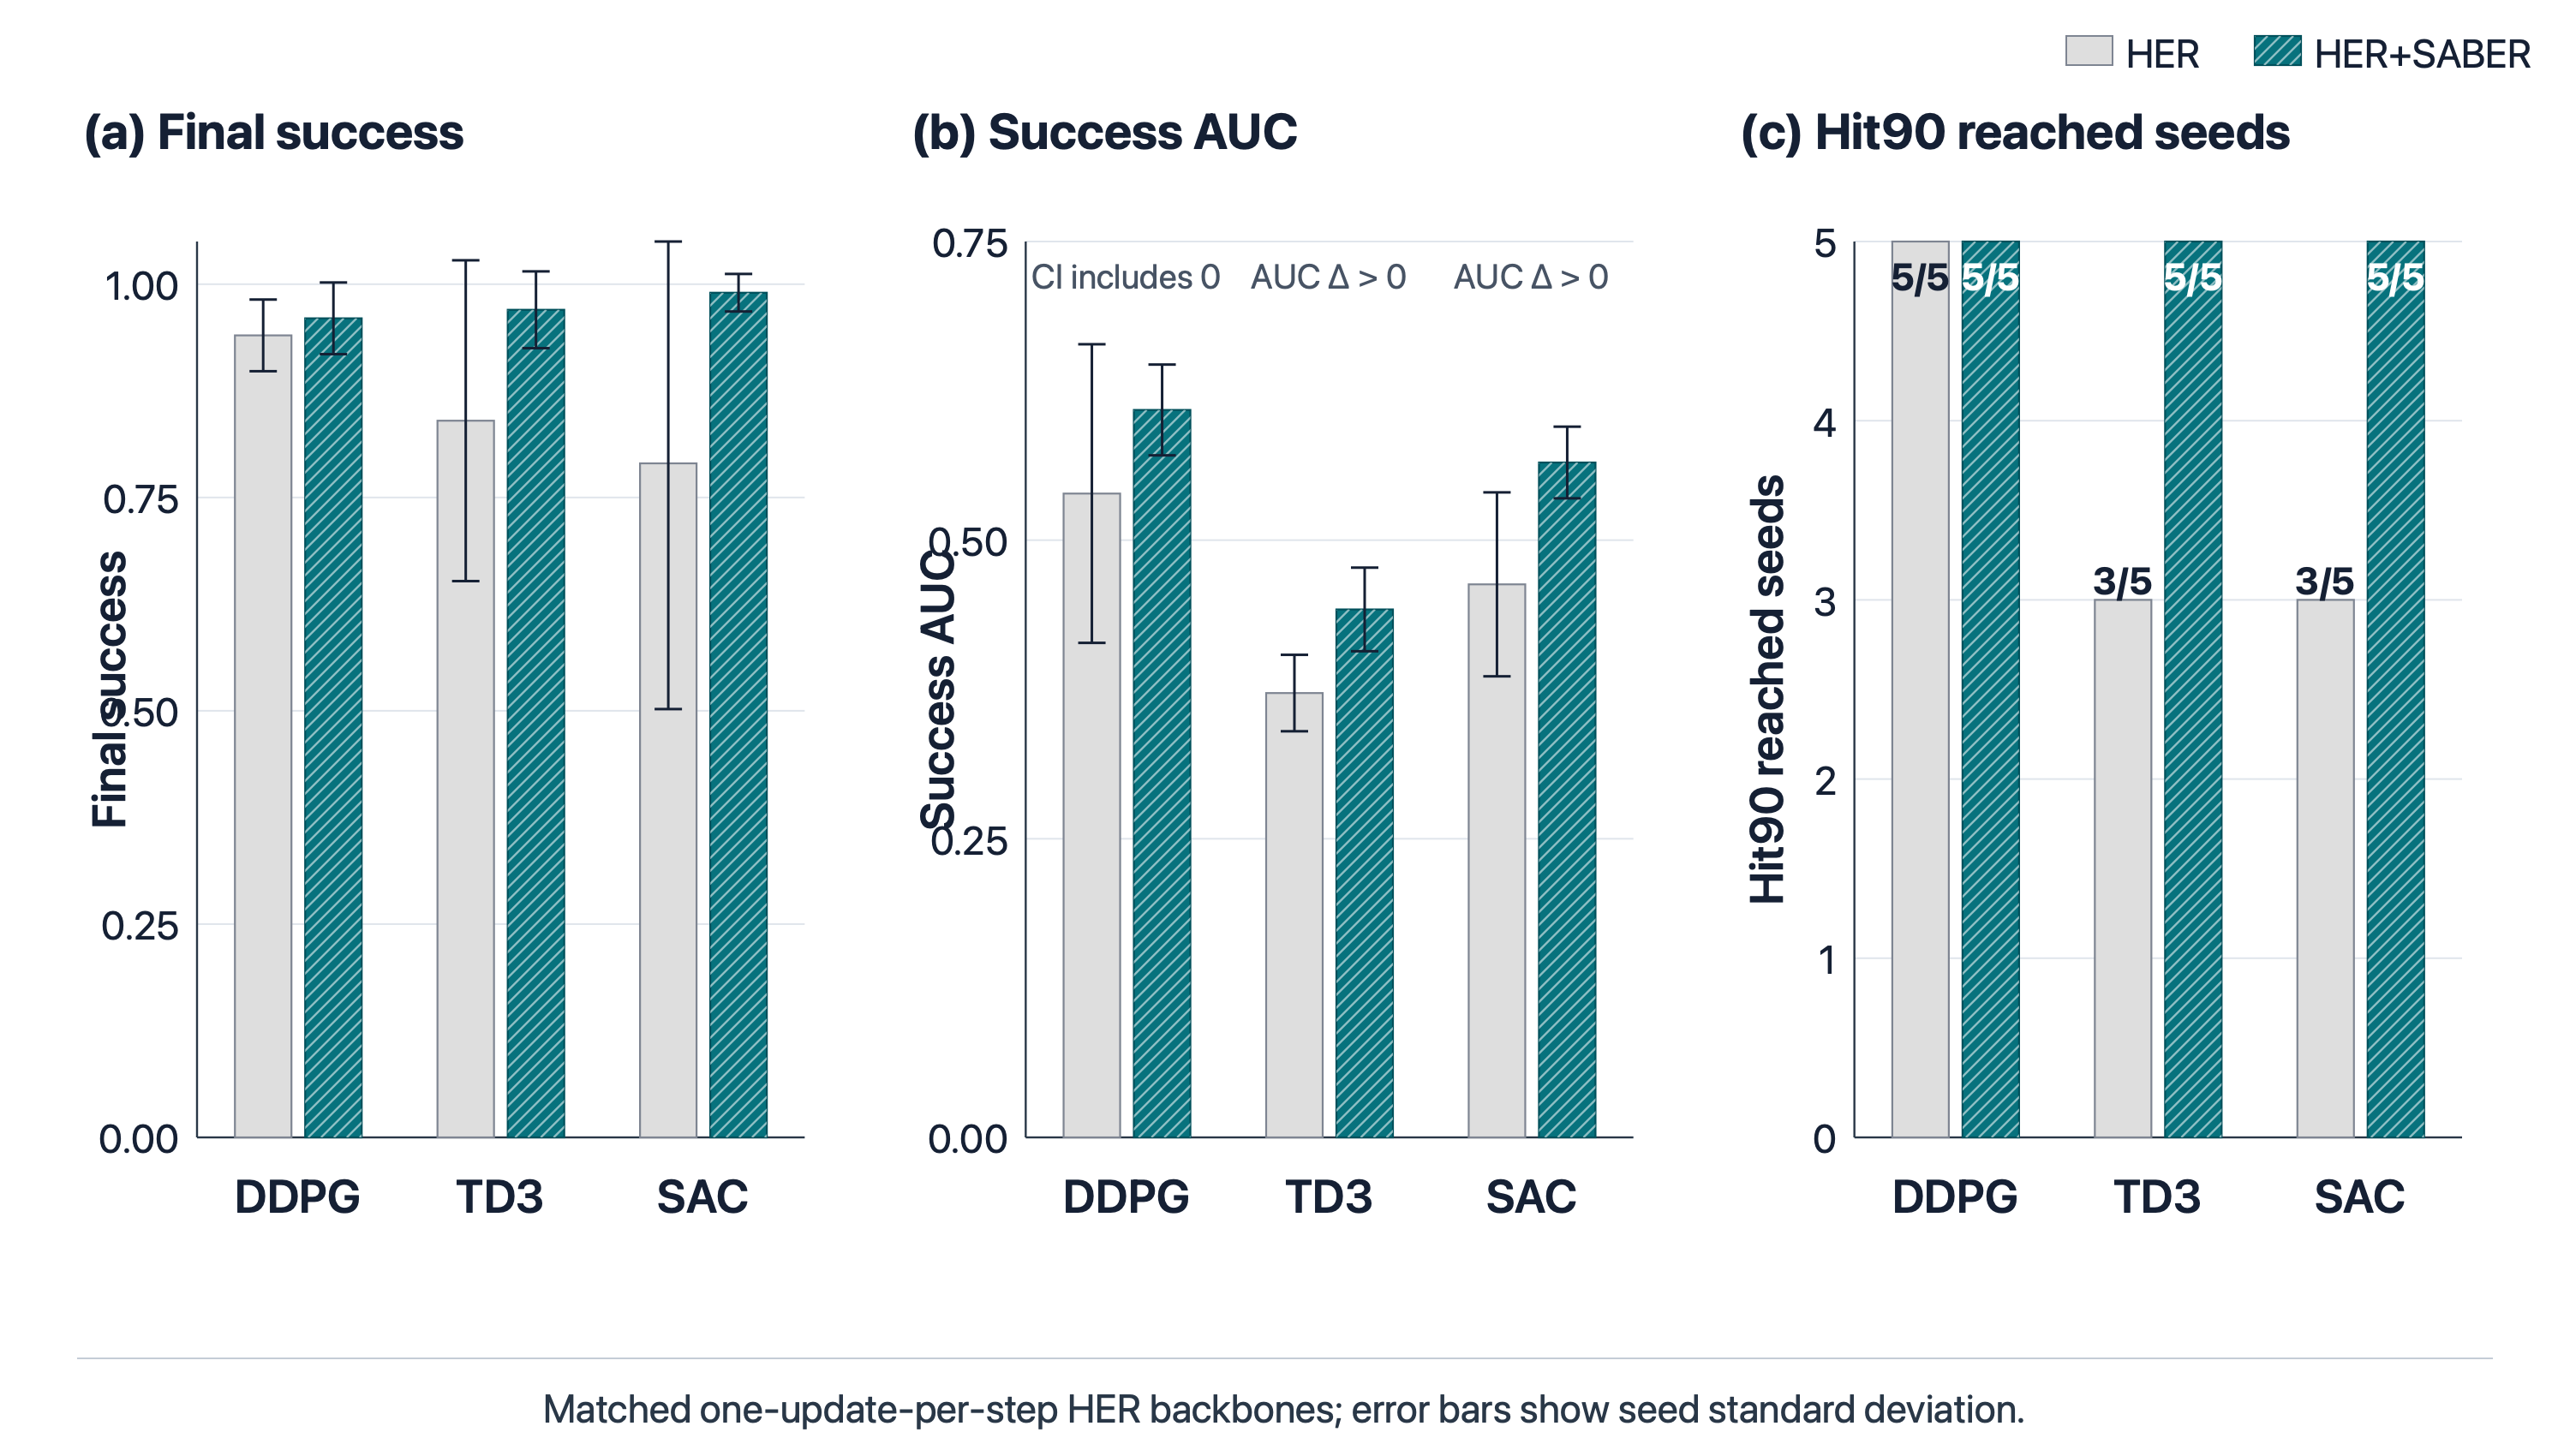
\includegraphics[width=0.98\textwidth]{output/figures/fpp_saber_main_evidence.png}
\caption{FetchPickAndPlace evidence across matched one-update-per-step HER backbones. Bars and error bars show the seed mean and standard deviation. Exact paired 95\% SABER--HER intervals are reported in Table~\ref{tab:fpp-main-submission}; the AUC interval includes zero for DDPG and excludes zero for TD3/SAC.}
\label{fig:fpp-main-evidence-submission}
\end{figure*}

\begin{table*}[t]
\centering
\small
\caption{Matched-backbone comparison: FPP main results and matched HGR reference at 1M steps. SAC AUC and Hit90 use the exact shared 50k--1M grid. SABER improves means across all backbones; paired AUC CIs are clearer for TD3/SAC than DDPG.}
\label{tab:fpp-main-submission}
\begin{tabular}{llcccc}
\toprule
Backbone & Method & Final & AUC & Hit90 & Steps/sec \\
\midrule
DDPG & HER & \(0.940 \pm 0.042\) & \(0.539 \pm 0.125\) & 600k (5/5) & \(65.03\) \\
\ourscell{DDPG} & \ours{HER+SABER} & \oursnum{0.960 \pm 0.042} & \oursnum{0.609 \pm 0.038} & \ourscell{540k (5/5)} & \oursnum{41.72} \\
DDPG & HGR (matched) & \(0.540 \pm 0.365\) & \(0.338 \pm 0.149\) & 930k (2/5) & \(16.93\) \\
TD3 & HER & \(0.840 \pm 0.188\) & \(0.372 \pm 0.032\) & 980k (3/5) & \(65.33\) \\
\ourscell{TD3} & \ours{HER+SABER} & \oursnum{0.970 \pm 0.045} & \oursnum{0.442 \pm 0.035} & \ourscell{840k (5/5)} & \oursnum{41.25} \\
SAC & HER & \(0.790 \pm 0.288\) & \(0.471 \pm 0.079\) & 800k (3/5) & \(38.93\) \\
\ourscell{SAC} & \ours{HER+SABER} & \oursnum{0.990 \pm 0.022} & \oursnum{0.583 \pm 0.030} & \ourscell{750k (5/5)} & \oursnum{29.10} \\
\midrule
DDPG & \(\Delta\) SABER--HER & \(+0.020[-0.040,0.070]\) & \(+0.070[-0.016,0.193]\) & -- & -- \\
TD3 & \(\Delta\) SABER--HER & \(+0.130[-0.030,0.310]\) & \(+0.071[0.032,0.095]\) & -- & -- \\
SAC & \(\Delta\) SABER--HER & \(+0.200[-0.020,0.430]\) & \(+0.112[0.064,0.161]\) & -- & -- \\
\bottomrule
\end{tabular}
\end{table*}

SABER raises mean FPP AUC from 0.539 to 0.609 on DDPG, 0.372 to 0.442 on TD3, and 0.471 to 0.583 on SAC. The paired AUC intervals exclude zero for TD3 and SAC, and all three backbones improve in mean final success and Hit90 coverage. This demonstrates cross-backbone compatibility rather than a single-backbone anomaly.

\paragraph{Ten-seed TD3 confirmation.}
A frozen paired extension on seeds 6--10 gives ten matched TD3 pairs on the exact 10k--1M grid. HER versus SABER reaches AUC $0.383\pm0.041$ versus $0.429\pm0.058$, with paired delta $+0.0467[0.0085,0.0783]$; 8/10 seed deltas are positive and every leave-one-out mean remains positive. The extension corroborates the five-seed result while preserving its finite-seed boundary: DDPG supplies mean-improvement rather than interval-closed evidence, and neither result implies improvement on every seed.

\subsection{Policy-Aligned Querying Is Substantive}

\textbf{The support query is not interchangeable with replay-action querying or sample-misaligned policy querying.}

\begin{table*}[t]
\centering
\small
\caption{FPP TD3 mechanism controls at 1M steps, seeds 1--5. Paired 95\% CIs compare Main with each row. The strict control samples \(k=|M|\) positions from \(E\) on each control update; context-count only is count-unmatched.}
\label{tab:query-ablation-submission}
\begin{tabular}{lcccc}
\toprule
Query / control & Final & AUC & Hit90 & Main $-$ row AUC [CI] \\
\midrule
HER & \(0.840\pm0.188\) & \(0.372\pm0.032\) & 980k (3/5) & \(+0.071[0.032,0.095]\) \\
\ours{Main SABER} & \oursnum{0.970\pm0.045} & \oursnum{0.442\pm0.035} & \ourscell{840k (5/5)} & \ourscell{--} \\
Replay action & \(0.660\pm0.219\) & \(0.368\pm0.042\) & 920k (1/5) & \(+0.075[0.059,0.092]\) \\
Shuffled policy & \(0.550\pm0.226\) & \(0.347\pm0.051\) & 890k (1/5) & \(+0.096[0.063,0.128]\) \\
\shortstack[l]{Context-eligible\\count-matched} & \(0.910\pm0.096\) & \(0.391\pm0.070\) & 955k (4/5) & \(+0.052[-0.016,0.099]\) \\
Context-count only & \(0.800\pm0.242\) & \(0.396\pm0.090\) & 850k (3/5) & \(+0.047[-0.041,0.122]\) \\
\bottomrule
\end{tabular}
\end{table*}

The main current-policy query exceeds replay-query and shuffled-policy on every paired seed. Replay-query has a higher support-positive rate than Main (0.426 versus 0.219) yet lower AUC, while shuffling preserves the policy-action marginal distribution but removes sample alignment. Thus query identity and sample alignment matter beyond merely producing more support-positive weights.

\textbf{Count-matched assignment.} Each control update recomputes \(E,M,k\) and samples \(Z\subseteq E\), \(|Z|=k\), without using membership locations; instrumented summaries record no count or weight-distribution violations. Main versus control AUC is \(0.4424\pm0.0350\) versus \(0.3908\pm0.0700\), with paired difference \(+0.0516[-0.0165,0.0992]\), 4/5 positive seeds, and exact \(p=0.25\). This removes the count confound and directionally favors membership alignment, but does not confirm its independent contribution.

\subsection{A Favorable Gradient-Update Trade-Off}

\textbf{On DDPG and TD3, SABER reaches AUC comparable to $4\times$ replay-ratio HER with one quarter of the gradient-update budget.}

\begin{table*}[t]
\centering
\small
\caption{Scaling references: FPP SAC/REDQ metrics use the exact shared 50k--1M grid. High-RR and REDQ rows expose update/backbone budget tradeoffs.}
\label{tab:scaling-submission}
\begin{tabular}{llccccc}
\toprule
Backbone & Method & Updates/step & Final & AUC & Hit90 & Runtime h \\
\midrule
\ourscell{DDPG} & \ours{HER+SABER} & \ourscell{1} & \oursnum{0.960 \pm 0.042} & \oursnum{0.609 \pm 0.038} & \ourscell{540k (5/5)} & \ourscell{6.66} \\
DDPG & HER high-RR \(4\times\) & 4 & \(0.990 \pm 0.022\) & \(0.618 \pm 0.071\) & 480k (5/5) & 16.11 \\
DDPG & HER high-RR \(8\times\) & 8 & \(0.720 \pm 0.407\) & \(0.443 \pm 0.269\) & 620k (3/5) & 31.85 \\
\ourscell{TD3} & \ours{HER+SABER} & \ourscell{1} & \oursnum{0.970 \pm 0.045} & \oursnum{0.442 \pm 0.035} & \ourscell{840k (5/5)} & \ourscell{6.74} \\
TD3 & HER high-RR \(4\times\) & 4 & \(0.610 \pm 0.243\) & \(0.449 \pm 0.079\) & 630k (1/5) & 8.76 \\
\ourscell{SAC} & \ours{HER+SABER} & \ourscell{1} & \oursnum{0.990 \pm 0.022} & \oursnum{0.583 \pm 0.030} & \ourscell{750k (5/5)} & \ourscell{9.55} \\
SAC & HER high-RR \(4\times\) & 4 & \(0.960 \pm 0.042\) & \(0.768 \pm 0.097\) & 450k (5/5) & 47.02 \\
REDQ-SAC & REDQ-HER TQB & 4 & \(1.000 \pm 0.000\) & \(0.867 \pm 0.052\) & 300k (5/5) & 89.52 \\
\bottomrule
\end{tabular}
\end{table*}

For TD3, comparable AUC is accompanied by substantially higher final success (0.970 versus 0.610) and Hit90 coverage (5/5 versus 1/5). SABER therefore offers a complementary one-update allocation strategy rather than relying on brute-force replay scaling. \textbf{Boundary:} this is a gradient-update trade-off, not a wall-clock-efficiency claim; SAC high-RR and REDQ-HER TQB attain higher AUC with larger update or architecture budgets.

\subsection{Large-Effect Rescue on DrawerOpen}

\textbf{SABER rescues a failure-prone HER regime on DrawerOpen.} It raises final success from 0.390 to 1.000, AUC from 0.207 to 0.754, and Hit90 coverage from 2/5 to 5/5 seeds. This shows that critic-side allocation can have a large practical effect when matched HER suffers from seed-level failures.

\begin{table*}[t]
\centering
\small
\caption{DrawerOpen stress case at 2M steps. DDPG rows use the local matched regime; REDQ-HER TQB is an N=10, M=2, UTD-4 architecture/compute-scaled reference. Hit90 reports median first hit and reached seeds.}
\label{tab:drawer-hgr-submission}
\begin{tabular}{lccc}
\toprule
Method & Final & AUC & Hit90 \\
\midrule
HER & \(0.390\pm0.534\) & \(0.207\pm0.287\) & 960k (2/5) \\
HGR-style sampler-only & \(0.400\pm0.548\) & \(0.311\pm0.425\) & 450k (2/5) \\
\ours{HER+SABER} & \oursnum{1.000\pm0.000} & \oursnum{0.754\pm0.044} & \ourscell{500k (5/5)} \\
Random-support & \(1.000\pm0.000\) & \(0.706\pm0.122\) & 510k (5/5) \\
PER-style & \(0.800\pm0.447\) & \(0.715\pm0.090\) & 610k (5/5) \\
REDQ-HER TQB (scaled) & \(1.000\pm0.000\) & \(0.672\pm0.314\) & 370k (5/5) \\
\bottomrule
\end{tabular}
\end{table*}

Random-support and PER-style controls are also strong, so DrawerOpen establishes intervention-family significance rather than unique structured-support causality. The HGR-style sampler-only row reaches Hit90 in 2/5 seeds; SABER minus HGR-style is \(+0.443[0.106,0.780]\) in AUC, but the row is not full HGR. Scaled REDQ-HER TQB reaches Hit90 earlier (370k versus 500k median), whereas SABER has higher mean AUC and lower variance, \(0.754\pm0.044\) versus \(0.672\pm0.314\); neither method dominates every seed or metric.

An independent SABER-only extension reaches Hit90 in 4/5 additional seeds; descriptively pooled over seeds 1--10, SABER reaches 9/10 with final success \(0.895\pm0.315\) and AUC \(0.652\pm0.246\). Because no matched methods were extended, the original five-seed paired comparisons remain primary. A separate diagnostic rerun reproduces the original five-seed aggregate AUC (0.755 versus 0.754). Across nine successful diagnostic seeds, support-positive samples show 1.17\(\times\) pre-update TD error and 2.1\(\times\) same-minibatch residual reduction; failed seed 7 first loses contact exploration and later exhibits support saturation. These in-sample diagnostics characterize allocation and failure behavior rather than causal generalization.

\begin{table*}[t]
\centering
\small
\caption{Control closure: what the reported controls establish and what remains unresolved.}
\label{tab:closure-submission}
\begin{tabular}{p{0.29\textwidth}p{0.31\textwidth}p{0.31\textwidth}}
\toprule
Evidence & Established & Remaining interpretation \\
\midrule
DDPG controls: Random-fixed AUC 0.540 is close to HER 0.539; Random-support AUC 0.604 is close to SABER 0.609. &
Fixed-count random weighting alone does not explain the gain. &
FPP DDPG does not isolate exact sample-level alignment; count-preserving randomization can regularize. \\
\addlinespace
TD3/SAC random controls stay near or below SABER in AUC. &
Random reweighting does not explain all gains across backbones. &
TD3/SAC provide the cleanest random-control separation. \\
\addlinespace
High-RR/REDQ rows match or exceed SABER under larger budgets. &
SABER offers a distinct one-update allocation strategy. &
It does not dominate update or architecture scaling. \\
\addlinespace
FPP HGR (matched) uses pair priorities and episode/pair IS correction but reaches AUC 0.338 and Hit90 in 2/5; SABER reaches 0.609 and 5/5. &
Matched goal prioritization does not explain SABER's gain in this regime. &
This is not an exact original-paper reproduction or a general HGR ranking. \\
\addlinespace
Diagnostics show weak TD-error correlation, top-error enrichment, and larger immediate correction in TD3/SAC. &
SABER is not PER-style largest-error selection. &
The evidence supports error allocation, not lower target variance. \\
\addlinespace
Main query AUC 0.442 exceeds replay 0.368 and shuffled 0.347 on all five paired seeds; the context-eligible count-matched control reaches 0.391. &
Current-policy identity and sample alignment are substantive, and the strict control removes the positive-count/context-eligibility confound. &
Main--control is \(+0.052[-0.016,0.099]\) on 4/5 seeds; membership-specific benefit is directional but not interval-closed. \\
\bottomrule
\end{tabular}
\end{table*}

\FloatBarrier
\raggedbottom
\subsection{Mechanism Characterization and Boundaries}

\paragraph{Allocation diagnostics.}
Instrumented DDPG, TD3, and SAC runs log 500 full diagnostic batches and 64k sample rows per backbone. Support-positive rates are 0.367, 0.219, and 0.197, while Pearson correlations with \(|\delta|\) are only 0.116, 0.128, and 0.143. Their top-10\% TD-error overlaps are 0.516, 0.360, and 0.342: enriched over each support base rate but far from TD-error equivalence. TD3/SAC support-positive samples also receive larger immediate residual correction after weight normalization. Target variance is higher, not lower, in all three diagnostics, supporting an allocation signal rather than a lower-noise interpretation.

Together, the controls establish a distinct policy-aligned allocation signal on TD3/SAC and characterize where generic reweighting, goal prioritization, or scaling remain competitive. They define the operating regime of the contribution rather than displacing its core matched-budget findings.

\section{Discussion}

\subsection{What SABER Establishes}

SABER establishes post-HER critic supervision allocation as a distinct design axis. Holding relabeling, replay, actor optimization, Bellman targets, critic architecture, and update rate fixed provides cleaner effect attribution and a common interface across DDPG, TD3, and SAC. The evidence then localizes the signal: aligned current-policy querying exceeds replay and shuffled-policy queries, cross-backbone and ten-seed results show repeatability, DDPG/TD3 expose a favorable gradient-update trade-off, and DrawerOpen demonstrates that critic-side allocation can rescue a failure-prone HER regime.

\subsection{Scope and Limitations}

The evidence is scoped in five ways. First, the support predicate is task-specific and uses coarse membership; FetchSlide DDPG decreases from HER final/AUC \(0.630/0.324\) to SABER \(0.590/0.301\), and DrawerClose remains high variance. Second, query and membership assignment are tested only on FPP TD3. The strict context-eligible count-matched control removes the earlier count confound and favors Main in mean AUC, but its five-seed interval includes zero; a weakly active D8 gate also does not establish a diversity benefit. Third, diagnostics are in-sample allocation measurements, not lower-noise or causal-generalization proofs. Fourth, the current lookup is costly: in a hardware-specific seed-1 profile, TD3 throughput falls from 124.0 to 41.4 steps/s and support/weighting occupies 62.3\% of SABER's loop. Fifth, matched FPP HGR is not an exact original-paper reproduction, HGG/MHER/CHER remain untested, and most controls use five seeds.

\paragraph{Statistical scope.}
Paired deltas use 10,000 seed bootstrap resamples. Exact sign-flip tests for FPP DDPG/TD3/SAC AUC give $p=0.375/0.125/0.0625$, with positive deltas on 3/5, 4/5, and 5/5 seeds; all leave-one-out means remain positive. With five nonzero pairs, 0.0625 is the minimum attainable two-sided value. The ten-seed TD3 extension contains two negative deltas and exact $p=0.0527$, while the DrawerOpen extension is SABER-only and unmatched. These checks establish repeatability and outlier stability, not improvement on every seed.

\section{Conclusion}
SABER establishes post-HER critic supervision allocation as a design axis distinct from relabeling, replay, actor optimization, Bellman targets, architecture, and update rate. It yields a repeatable cross-backbone FPP signal, corroborated by the paired TD3 ten-seed extension, and aligned current-policy querying outperforms replay/shuffled alternatives. Count matching removes the earlier confound but does not interval-close the incremental membership effect. SABER also offers a DDPG/TD3 gradient-update trade-off and rescues a failure-prone DrawerOpen regime. Generic support representations remain future work.

\section{Reproducibility and Anonymity}

An anonymized archive provides sanitized configs, exact-grid curves, package-local analyzers/tests, and SHA256 manifests for the matched HGR, TD3 ten-seed, query/count-matched, DrawerOpen, scaling, and runtime evidence. Package commands regenerate compact tables; independent checks cover exact inference, leave-one-out, and table consistency. Public URLs, user namespaces, and raw commit identities are excluded.

\makeatletter
\@ifundefined{isChecklistMainFile}{\bibliographystyle{aaai2027}}{}
\makeatother
\bibliography{saber_refs}

\end{document}
